\section{Morphology-Dependent Failure Analysis}

Unknown rejection difficulty varies strongly by morphology. This is visible in both internal analyses and external AML-LMU results. The practical implication is that a single aggregate AUROC can hide qualitatively different failure modes. Some unknown classes are rejected with relatively high AUROC, while others are repeatedly absorbed by a semantically related known class.

\subsection{External Unknown Morphologies}

Under the external CE+ViM analysis, the easiest unknown morphologies by mean AUROC are promyelocyte (0.897), myelocyte (0.880), metamyelocyte (0.867), promyelocyte-bilobled (0.856), and erythroblast (0.792). The hardest are neutrophil-band (0.526), monoblast (0.575), myeloblast (0.592), lymphocyte-atypical (0.597), and smudge-cell (0.782). The associated FPR@95TPR values are especially high for neutrophil-band (0.944) and myeloblast (0.819). These values are morphology-specific open-set results, not clinical difficulty rankings.

\subsection{Attractor Behavior}

The hardest classes align with known-class attractors. External neutrophil-band images have segmented neutrophil as the dominant known prediction in all CE+ViM external runs. Monoblast maps dominantly to monocyte. Myeloblast, lymphocyte-atypical, and smudge-cell often map to lymphocyte. This indicates that unknown errors are not uniformly distributed. They cluster along morphologically plausible known-class neighborhoods, which helps explain why high closed-set classification accuracy can coexist with weak rejection.

\subsection{Neutrophil Band and Lymphoid-Like Cases}

Neutrophil-band is the clearest persistent failure family. In internal Delivery 6, ArcFace consistently degraded MSP rejection of neutrophil-band, with mean AUROC deltas of -0.120 on V1 and -0.112 on V2, and zero of five favorable seeds in both split protocols. In the external analysis, the same class remains difficult for CE+ViM, with AUROC 0.526 and FPR@95TPR 0.944. ViM improves band-neutrophil AUROC for ArcFace in the dedicated case summary, but that improvement does not make ViM the best external method overall.

Lymphoid-like unknowns show a different pattern. Large granular lymphocyte, neoplastic lymphocyte, reactive lymphocyte, and hairy-cell morphologies retain high attraction to the known lymphocyte class. For large granular lymphocyte, the mean attraction to lymphocyte is 0.972 under CE and 0.978 under ArcFace. ArcFace improves some MSP AUROCs in this family, but attraction remains high. Thus, a better rejection score in selected cases does not necessarily imply a disentangled representation.

\begin{figure}[htbp]
\centering
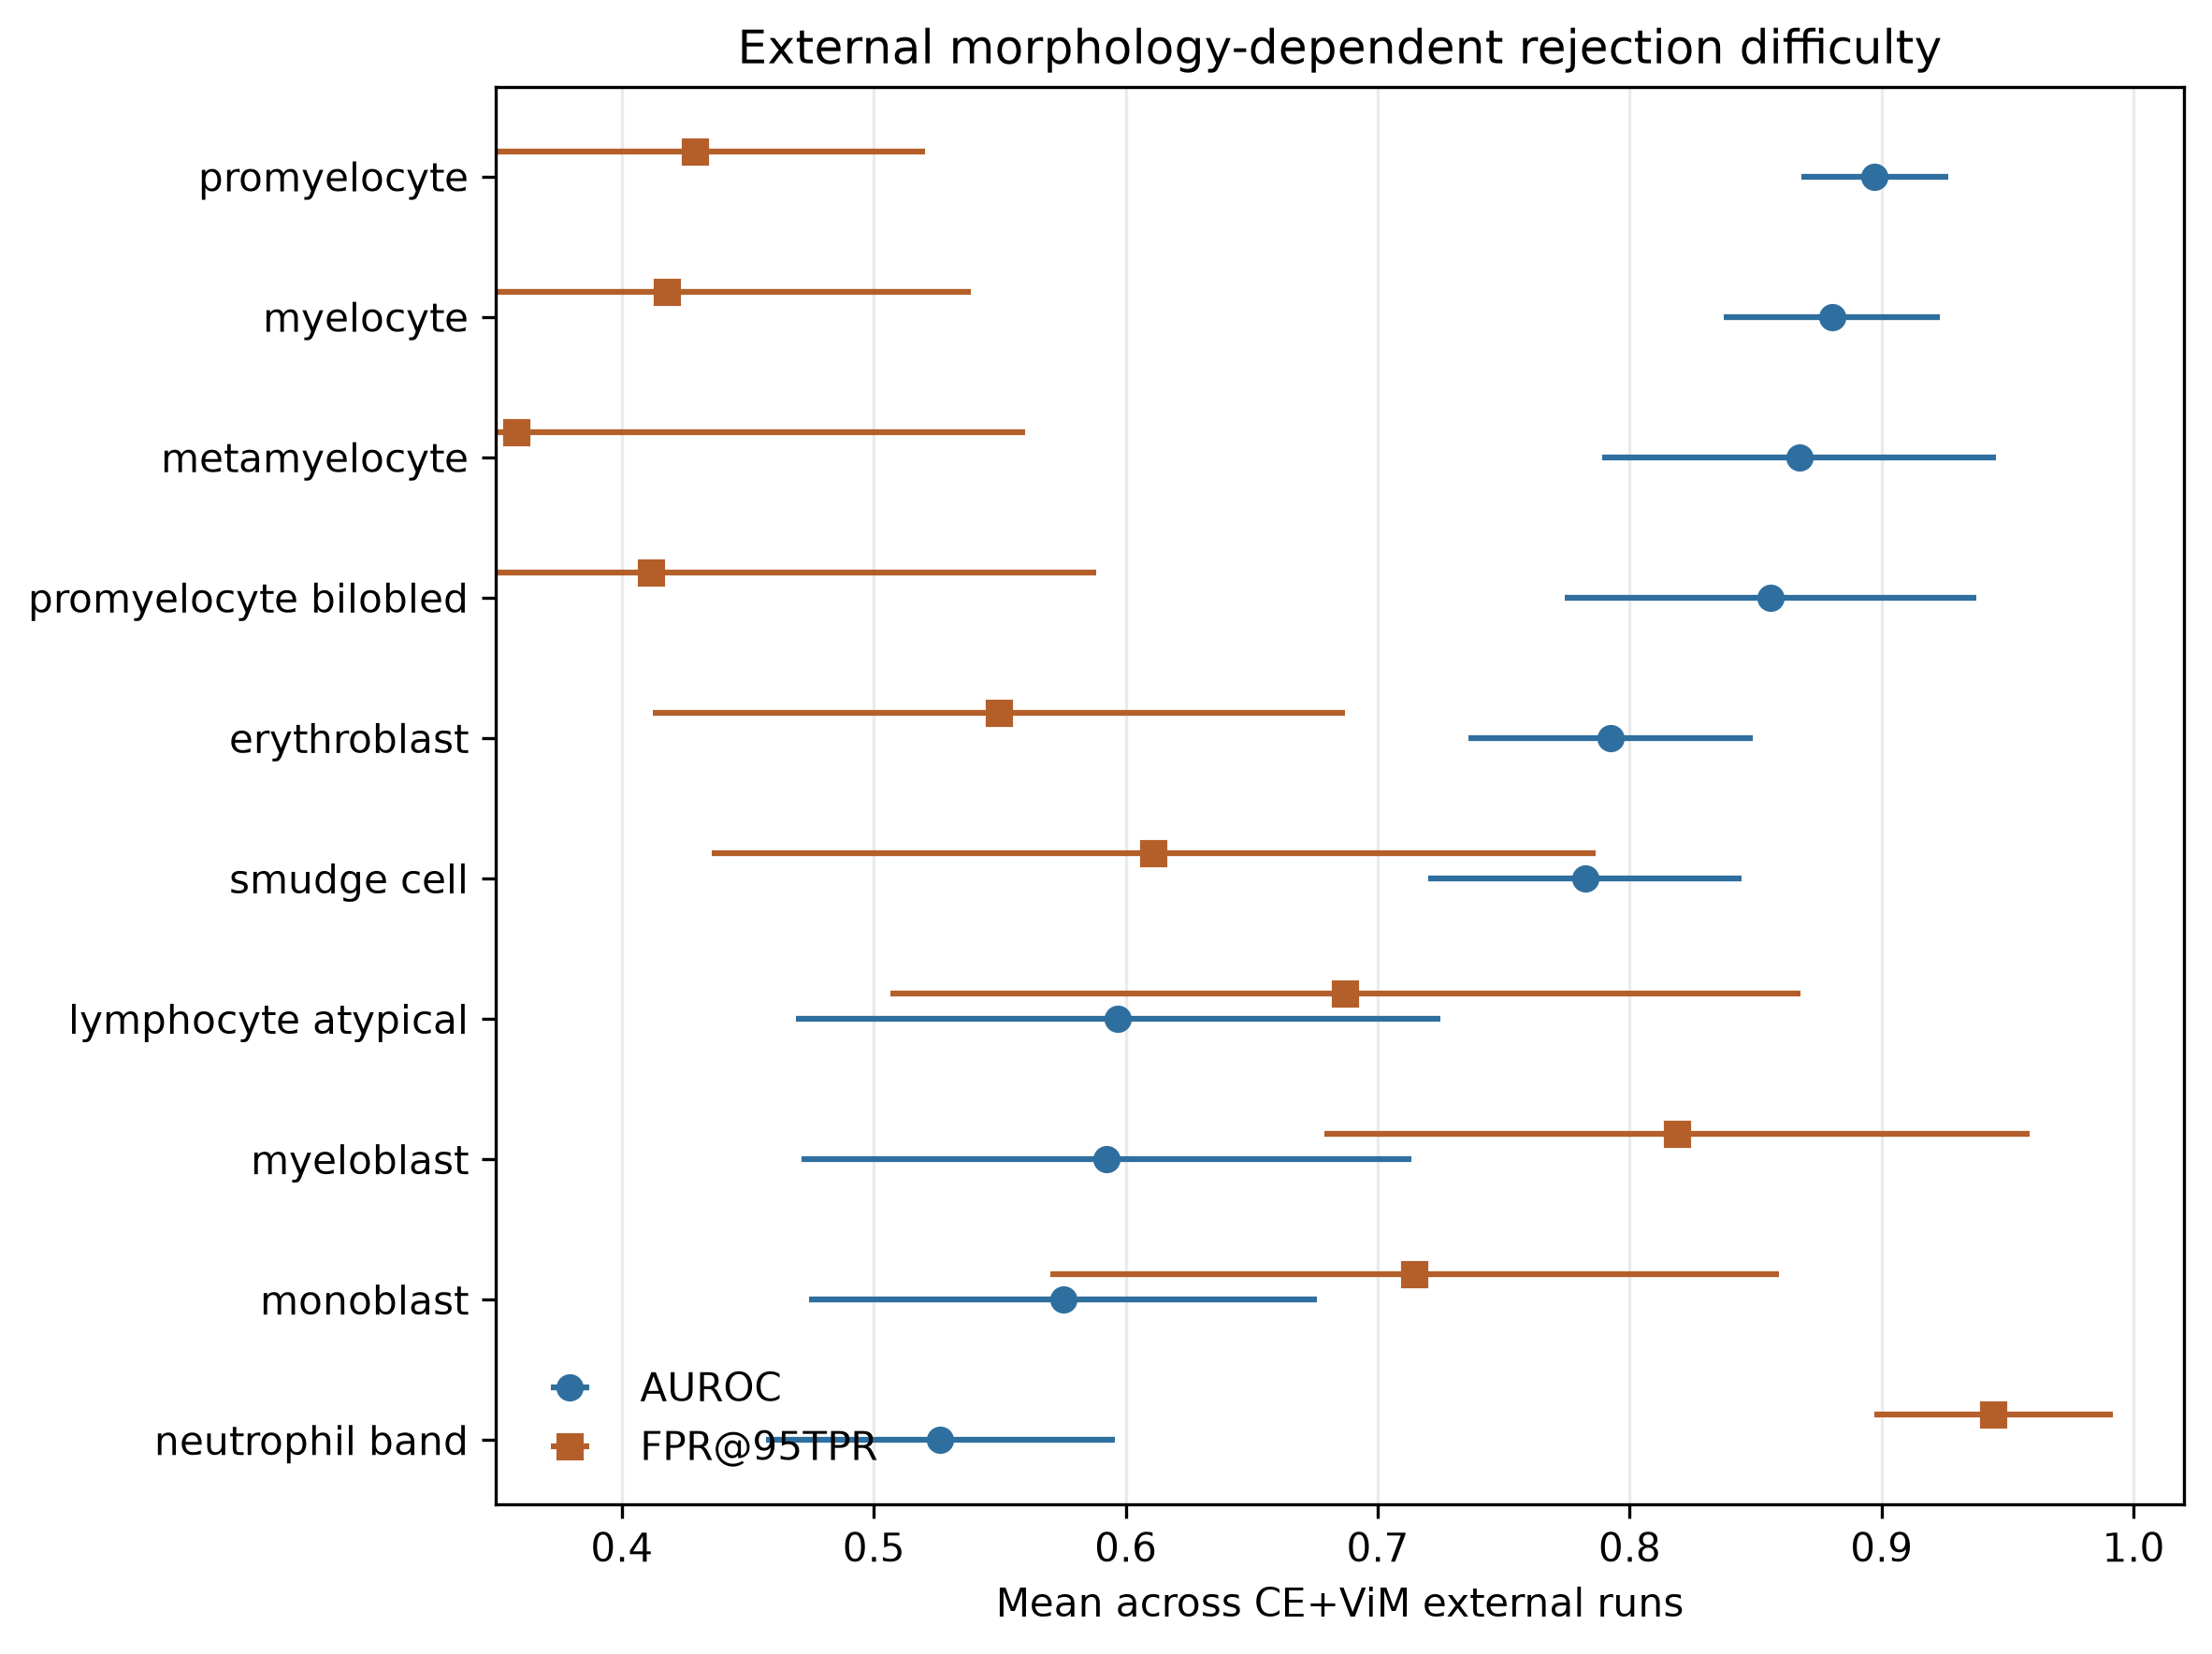
\includegraphics[width=0.86\textwidth]{figures/figure5_external_morphology.png}
\caption{External morphology-dependent unknown detection for CE+ViM. Error bars show standard deviation across external CE+ViM runs.}
\label{fig:external-morphology}
\end{figure}

\begin{figure}[htbp]
\centering
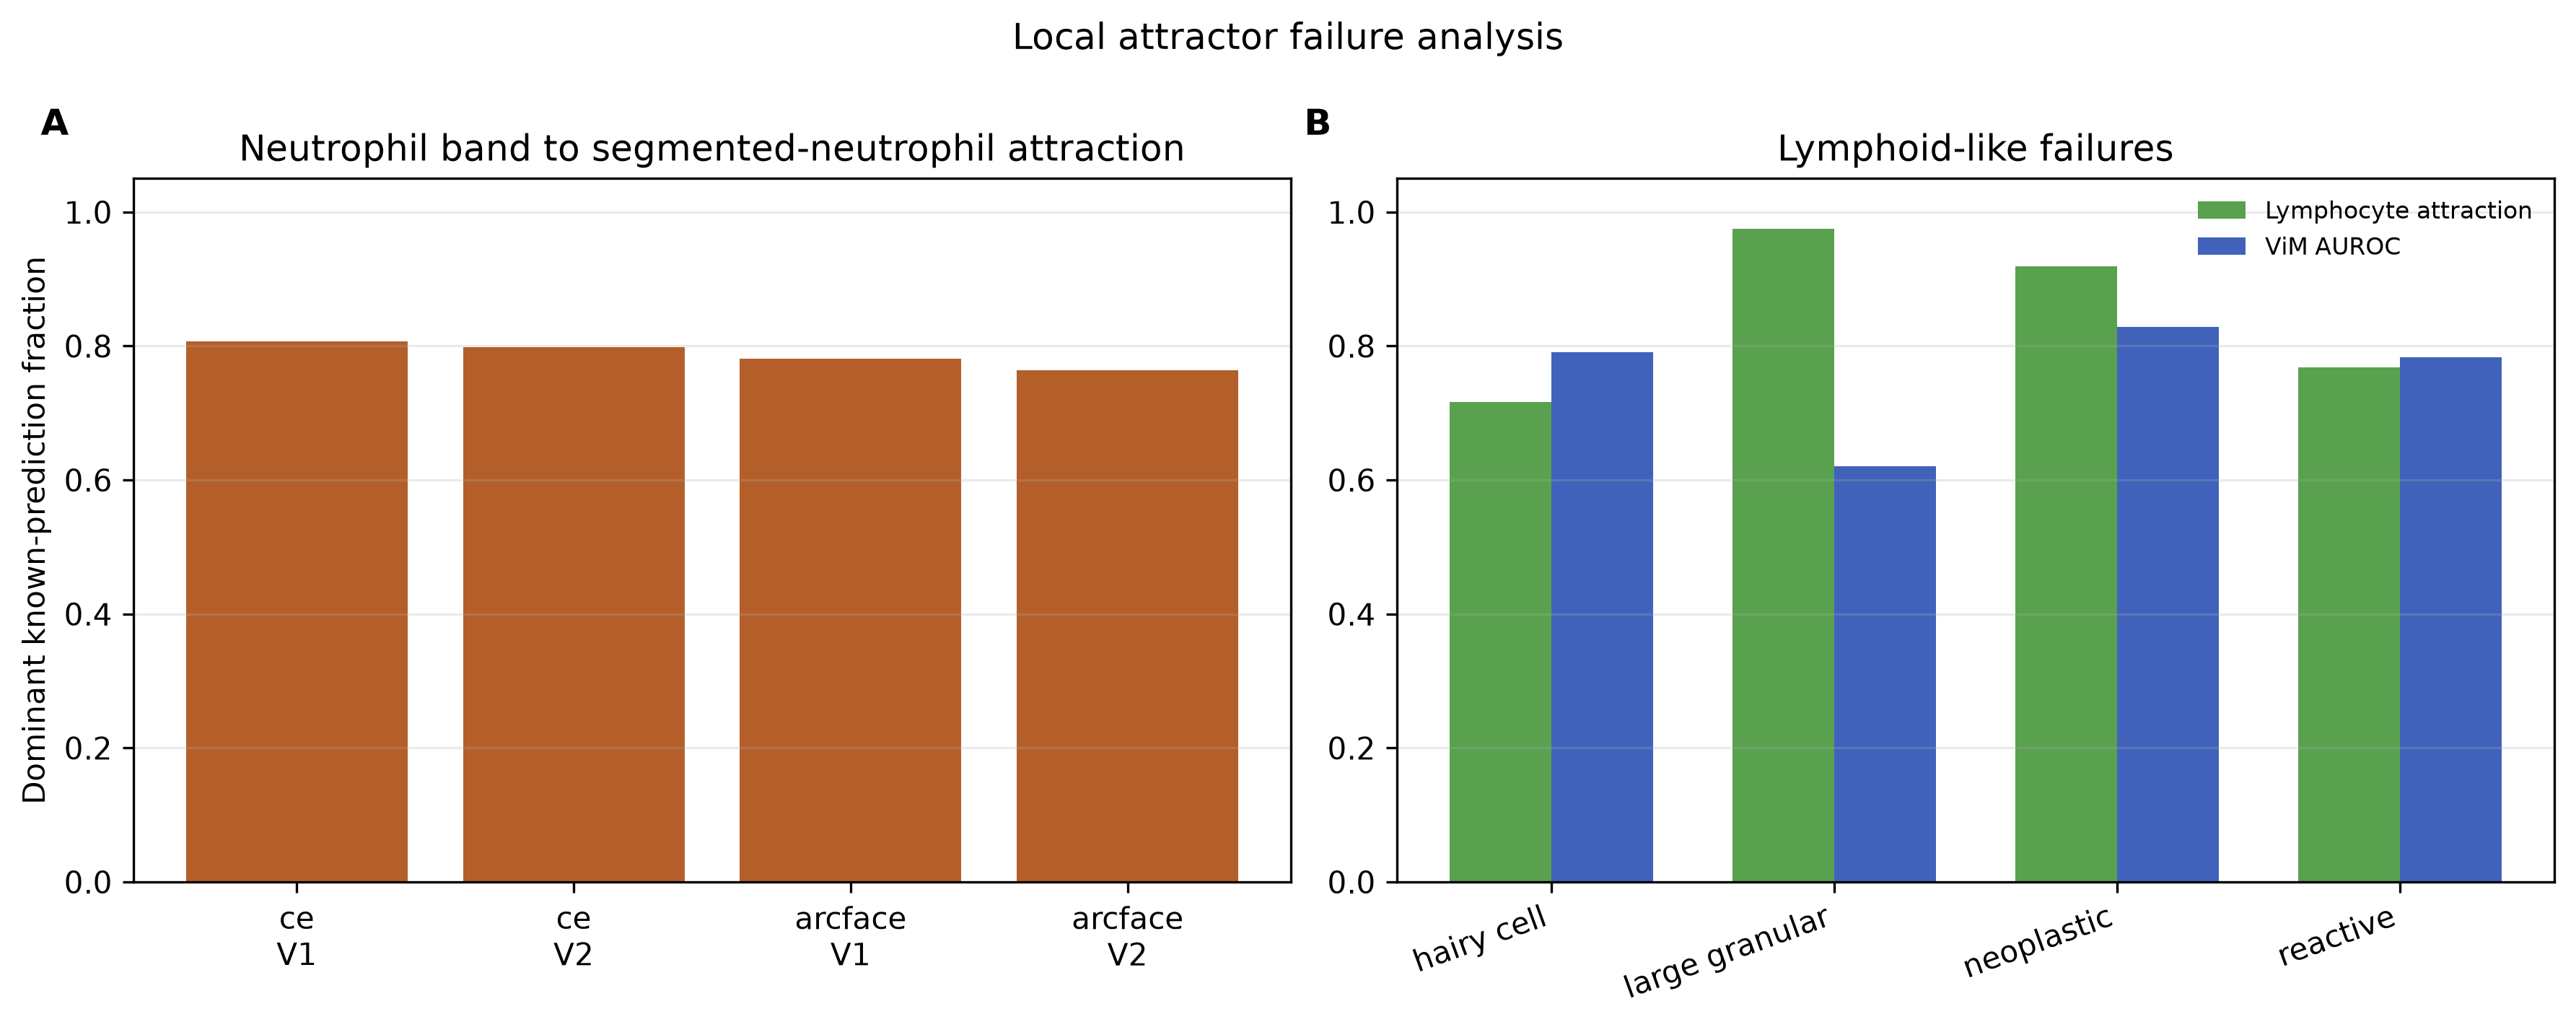
\includegraphics[width=\textwidth]{figures/figure6_failure_cases.png}
\caption{Known-class attractor failure analysis for neutrophil-band and lymphoid-like unknown morphologies.}
\label{fig:failure-cases}
\end{figure}
